\documentclass[conference]{IEEEtran}
% \IEEEoverridecommandlockouts
% The preceding line is only needed to identify funding in the first footnote. If that is unneeded, please comment it out.
\usepackage{cite}
\usepackage{amsmath,amssymb,amsfonts}
\usepackage{algorithmic}
\usepackage{graphicx}
\usepackage{textcomp}
\usepackage{xcolor}
\usepackage{colortbl}
\usepackage{xspace}
\usepackage[hidelinks]{hyperref}
\usepackage[a4paper, total={184mm,239mm}]{geometry}

\usepackage{pifont}
\newcommand{\gcheck}{\ding{51}} % ✓
\newcommand{\rcross}{\ding{55}} % ✗

\def\BibTeX{{\rm B\kern-.05em{\sc i\kern-.025em b}\kern-.08em
    T\kern-.1667em\lower.7ex\hbox{E}\kern-.125emX}}

%%%%%%%%%%%%%%%%%%%%%%%%%%%%%%%%%%%%%%%%%%%%%%%%%%%%%%%%%%%%%%%%%%%%%%%%%%%%%%%%%%%%%%
%     __________  ____  ____     _   ______  _________________
%    /_  __/ __ \/ __ \/ __ \   / | / / __ \/_  __/ ____/ ___/
%     / / / / / / / / / / / /  /  |/ / / / / / / / __/  \__ \
%    / / / /_/ / /_/ / /_/ /  / /|  / /_/ / / / / /___ ___/ /
%   /_/  \____/_____/\____/  /_/ |_/\____/ /_/ /_____//____/
%
% Thanks Patrick-san for the snippet
\usepackage{ifthen}
\newboolean{EnableTodoNotes}
\setboolean{EnableTodoNotes}{true}  % <<< set this to "false" to disable todos
\ifthenelse{\boolean{EnableTodoNotes}}{%
  \usepackage[colorinlistoftodos,prependcaption,obeyFinal,textsize=footnotesize]{todonotes}
  \paperwidth=\dimexpr \paperwidth + 6cm\relax
  \oddsidemargin=\dimexpr\oddsidemargin + 3cm\relax
  \evensidemargin=\dimexpr\evensidemargin + 3cm\relax
  \marginparwidth=\dimexpr \marginparwidth + 3cm\relax
}{%
  \usepackage[colorinlistoftodos,prependcaption,obeyFinal,disable]{todonotes}
}
\newcommand{\cf}[1]{\todo[color=pink!40]{\textbf{CF}: #1}}
\newcommand{\fls}[1]{\todo[color=cyan!40]{\textbf{FS}: #1}}


\begin{document}

\newcommand{\para}[1]{\vspace{0.6\baselineskip}\noindent\textbf{#1.}}
% \newcommand{\para}[1]{\vspace{0.3\baselineskip}\noindent\textbf{#1.}}

\newcommand{\Pic}{Platform timing contract\xspace}
\newcommand{\pic}{platform timing contract\xspace}
\newcommand{\Pics}{Platform timing contracts\xspace}
\newcommand{\pics}{platform timing contracts\xspace}
\newcommand{\pici}{platform timing contract instrumentation\xspace}
\newcommand{\Pici}{Platform timing contract instrumentation\xspace}
\newcommand{\PICI}{PTCI\xspace}
\newcommand{\PICIs}{PTCIs\xspace}
\newcommand{\ucfi}{$\mu$CFI\xspace}

\title{Platform Timing Contracts: A Lightweight Instrumentation for Capturing SoC Timing Channels}

% \author{\IEEEauthorblockN{1\textsuperscript{st} Given Name Surname}
% \IEEEauthorblockA{\textit{dept. name of organization (of Aff.)} \\
% \textit{name of organization (of Aff.)}\\
% City, Country \\
% email address or ORCID}
% \and
% \IEEEauthorblockN{2\textsuperscript{nd} Given Name Surname}
% \IEEEauthorblockA{\textit{dept. name of organization (of Aff.)} \\
% \textit{name of organization (of Aff.)}\\
% City, Country \\
% email address or ORCID}
% \and
% \IEEEauthorblockN{3\textsuperscript{rd} Given Name Surname}
% \IEEEauthorblockA{\textit{dept. name of organization (of Aff.)} \\
% \textit{name of organization (of Aff.)}\\
% City, Country \\
% email address or ORCID}
% \and
% \IEEEauthorblockN{4\textsuperscript{th} Given Name Surname}
% \IEEEauthorblockA{\textit{dept. name of organization (of Aff.)} \\
% \textit{name of organization (of Aff.)}\\
% City, Country \\
% email address or ORCID}
% \and
% \IEEEauthorblockN{5\textsuperscript{th} Given Name Surname}
% \IEEEauthorblockA{\textit{dept. name of organization (of Aff.)} \\
% \textit{name of organization (of Aff.)}\\
% City, Country \\
% email address or ORCID}
% \and
% \IEEEauthorblockN{6\textsuperscript{th} Given Name Surname}
% \IEEEauthorblockA{\textit{dept. name of organization (of Aff.)} \\
% \textit{name of organization (of Aff.)}\\
% City, Country \\
% email address or ORCID}
% }

\maketitle

\begin{abstract}
Variations in the time a computer requires to perform computations can leak confidential information.
Constant-time programming techniques defend against such timing attacks, but make assumptions on the behavior of the underlying hardware.
As a response, previous work has introduced several techniques for verifying CPU compliance with hardware-software contracts.
%
However, selecting which hardware-software contract to verify is non-trivial and requires careful consideration of the system's architecture and the specific timing attacks it may face.
If a CPU is integrated into a platform with more timing channels than expected, CPU verification alone may be insufficient to guarantee security.
In this paper, we address the integration of a verified constant-time CPU into a larger system.
We make three contributions: (1) we define \pics as a formal way to capture an upper bound of the platform-induced timing channels, (2) we design a low-overhead synthetizable instrumentation that materializes these contracts and is compatible with all existing CPU verification methods, and (3) we demonstrate that existing CPU verification techniques along fail under integration, whereas \pics enable stronger, system-wide security guarantees against timing attacks.

% We introduce platform timing contracts, a novel abstraction that specifies an upper bound on timing channels introduced by platform integration.
% We introduce a lightweight instrumentation that allows for the dynamic monitoring of platform-induced timing channels and that is inherently compatible with all CPU constant-time verification techniques.
% Based on this instrumentation, we show that several techniques, while effective in isolation, fail to provide security guarantees when the CPU is integrated into a larger system.

\end{abstract}

% \begin{IEEEkeywords}
% component, formatting, style, styling, insert
% \end{IEEEkeywords}

%-------------------------------------------------------------------------------
\section{Introduction} \label{sec:introduction}
%-------------------------------------------------------------------------------
% !TeX root = ../main.tex
% !TeX spellcheck = en_US

\textcolor{red}{Should not only be about uarch. Should also be about archi leakage also?}
Microarchitectural attacks are software-driven techniques that exploit behaviors below the ISA to encode and reveal secrets through measurable side effects, most commonly execution time.
By carefully choreographing benign-looking instruction sequences, an attacker steers microarchitectural state, such as caches, TLBs, execution ports, branch predictors, DRAM buffers, to make secret-dependent effects externally observable.
Two broad families have emerged: transient/speculative-execution attacks~\cite{kocher2019spectre,lipp2018meltdown,armsecure,bhattacharyya2019smotherspectre,van2018foreshadow,canella2019fallout,horn2018speculative,maisuradze2018ret2spec,schwarz2019zombieload,schwarz2019netspectre,stecklina2018lazyfp,van2019ridl,ragab2021crosstalk,van2020lvi,van2021cacheout,ragab2021rage,wikner2022retbleed,trujillo2023inception,wikner2023phantom,wikner2024breaking,wikner2025bpi}, which leave secret-dependent footprints during mis-speculated execution, and contention-driven channels on shared resources~\cite{bernstein2005cache,bonneau2006cache,Liu2015LLC,YaromFalkner2014FlushReload,Gras2018TLBleed,Aldaya2019PortSmash,Yarom2016CacheBleed,Moghimi2018MemJam,Gruss2016PrefetchSCA,Pessl2016DRAMA}, which measure or induce interference to encode information.
These attacks pose a durable, cross-generation threat to modern processors, in particular because they can be mounted entirely in software, without special privileges or hardware access.
Mitigation is notoriously difficult once silicon has shipped: the leakage channels are entwined with performance-critical design choices.
Software or microcode defenses are often partial~\cite{ridlad} or impose significant overheads.

To inform software developers about the potential side effects of their code on a given contract-compliant CPU, recent work has introduced hardware-software contracts~\cite{guarnieri2021hardware,oleksenko2022revizor}.
As a result, several techniques have been proposed to formally verify that a CPU implementation complies with such contracts~\cite{dinesh2024conjunct,dinesh2025h,ceesay2024mucfi,wang2023specification,tan2025contractshadowlogic,hsiao2024rtl2mmupath} to prevent confidentiality breaches before chip fabrication.

\para{Platform timing channels}
CPUs are often verified in isolation~\cite{dinesh2024conjunct,dinesh2025h,ceesay2024mucfi,wang2023specification,tan2025contractshadowlogic,hsiao2024rtl2mmupath} before integration into a larger system, often for scalability reasons.
Yet hardware-software contracts make assumptions on the system into which a CPU will be integrated.
For example, the constant-time contract observer mode~\cite{guarnieri2021hardware} exposes the program counter of every executed instruction, and the addresses of all memory operations.
This observation mode accounts for the timing effects of caches and other elements of the memory hierarchy~\cite{guarnieri2021hardware,oleksenko2022revizor}.
Other contract observation modes exist, for example the architectural observer, which additionally discloses values exchanged with memory.
These aspects of hardware-contracts are proper to the platform (i.e., the broader SoC) into which the CPU will be integrated, yet many verification techniques do not account for them or provide this flexibility.

\para{Platform timing contracts}
Platform timing contracts extend the idea of hardware-software contracts to encompass the broader system context in which a CPU operates.
They aim to capture the timing behavior of the entire platform, including interactions with other components such as memory controllers, I/O devices, and interconnects.
By considering these interactions, platform timing contracts can provide a more comprehensive understanding of potential timing channels and their implications for security.
To verify the compliance of a CPU integrated into a specific platform using existing techniques that verify a CPU in isolation, we introduce an automatic instrumentation that captures the relevant platform-specific timing information while retaining compatibility with all existing hardware-software contract verification techniques.

We establish the platform timing contracts for \textcolor{red}{3} different platforms.
We apply the instrumentation corresponding to each platform to the \textcolor{red}{4} RISC-V CPUs \textcolor{red}{TODO List them}.
Not only does the verification time increase by not more than ~\textcolor{red}{5}\%, but we demonstrate the existence of platform-specific timing channels on typical platforms, that would otherwise be missed.

In summary, our contributions in this paper are:
\begin{itemize}
    \item We introduce \pics.
    \item We implement an open-source lightweight CPU instrumentation that accounts for all platform-induced timing side-channels.
    \item We apply instrumentations corresponding to various platforms to the 4 RISC-V CPUs to capture platform-specific timing information and show that these platforms can introduce unique timing channels that may not be present in isolated CPU verification and that would be missed by some existing verification techniques.
\end{itemize}

\vspace*{0.5em}
All our experiments can be found at: \url{https://placeholder/} 

% % TODO Say the importance of platform side channels.

% % Microarchitectural attacks exploit subtle CPU features to encode and leak sensitive information through program execution time. Because they can be mounted entirely from software, they pose a significant long-term threat to modern CPUs.
% % They may exploit speculative execution~\cite{kocher2019spectre,lipp2018meltdown,armsecure,bhattacharyya2019smotherspectre,van2018foreshadow,canella2019fallout,horn2018speculative,maisuradze2018ret2spec,schwarz2019zombieload,schwarz2019netspectre,stecklina2018lazyfp,van2019ridl,ragab2021crosstalk,van2020lvi,van2021cacheout,ragab2021rage} or resource contention~\cite{bernstein2005cache,bonneau2006cache,Liu2015LLC,YaromFalkner2014FlushReload,Gras2018TLBleed,Aldaya2019PortSmash,Yarom2016CacheBleed,Moghimi2018MemJam,Gruss2016PrefetchSCA,Pessl2016DRAMA}.
% % They are notoriously difficult to mitigate once hardware has been fabricated.

% Traditionally, these vulnerabilities were looked for manually~\cite{dessouky2019hardfails} or using dynamic techniques that are as good as their test cases~\cite{weber2021osiris,ghaniyoun2021introspectre,de2025phantom,hur2022specdoctor,rostami2024lost,borkar2024whisperfuzz,oleksenko2022revizor}.
% Recently, advances in speculation contracts~\cite{guarnieri2021hardware} and relational reasoning~\cite{oleksenko2022revizor} have formalized the problem of proving the absence of timing channels in CPUs as a \emph{non-interference} property.
% Intuitively, a CPU complies with such a non-interference property if the program's secret data does not affect the CPU's observable behavior, if the program complies with some understanding of constant-time property.
% For example, the program shall not use the secret data as the input to a branch if adversaries can observe branch decisions.
% Such program constraints can be understood as variants of constant-time programming.

% Several dedicated verification schemes have been proposed in the last few years.
% They formally prove the absence of an information leakage from secret data to observable channels such as timing, generally based on one of two properties named \emph{Safe Instruction Set} (SIS) and the stronger \emph{Speculative Non-Interference} (SNI).
% Despite being different properties, both guarantee that secret information computed in a CPU cannot be inferred from the system's observable behavior if the software is written in a constant-time manner.
% However, all the so-far-proposed techniques for formally proving constant-time properties in CPUs make explicit or implicit assumptions on the system into which the CPU will be integrated, and on the implementation of the CPU under verification or on the systems that integrate it.
% \fls{We might also say something about the threat model / about SoCs that have external IPs.}

% \para{\Pics}
% Some information flows that can reveal secrets might exit the CPU to reenter it and affect its timing, and might escape the scope of verification techniques through these reentrant paths. 
% The existence and nature of such reentrant information flows depend on the system into which the CPU is integrated.
% Yet, no existing constant-time verification technique addresses this issue explicitly.
% Some techniques ignore reentrant information flows altogether~\cite{ceesay2024mucfi,dinesh2024conjunct,dinesh2024conjunct}.
% We will see that this can lead to missing vulnerabilities that would be otherwise detectable when the CPU is integrated into a larger system.
% Others techniques may assume the existence of address-dependent timing channels~\cite{wang2023specification,tan2025contractshadowlogic}, due for example to caches present in the system.
% To address this issue, we introduce \pics, a simple specification of the reentrant information flows that exit and reenter the CPU.
% Based on this specification, we introduce an automatic lightweight instrumentation that augments a CPU with a synthesizable summary of all the potential reentrant information flows from the platform that integrates the CPU.

% \para{Assumptions in constant-time verification}
% We note that unsoundness is not only due to reentrant information flows, but also due to assumptions made by the verification techniques.
% We analyze the assumptions that underpin the automatic state-of-the-art non-interference property verification techniques, once the reentrant flow challenge is addressed.
% We find that these assumptions can be categorized into three classes.
% (a) The \emph{Correctness Assumption}: a CPU shall be exempt from functional bugs.
% % In this paper, we find that a well-defined class of functional correctness bugs, which are common even in widely-adopted CPUs~\cite{solt2022rememberr}, can cause unsoundness under this assumption.
% In this paper, we demonstrate that indeed functional correctness bugs can cause unsoundness for techniques that formulate this assumption.
% Further, we identify that only a well-defined class of functional correctness bugs can lead to such unsoundness.
% (b) The \emph{Architectural Flow Matching Assumption}: information flows on architectural paths shall coincide with architectural transactions.
% In this paper, we show that microarchitectural transactions that are not architectural, such as microarchitecturally reading architectural values during transient execution, can cause unsoundness for techniques that formulate this assumption.
% (c) The \emph{Input Constraint Assumption}: some input data words shall be constrained to a restricted set of potential values interpreted as safe instruction encodings.
% In this paper, we show that an increase in the diversity of input words, such as the cohabitation of data and instructions on a memory bus, is typical when the CPU is integrated into a larger system, and can cause unsoundness for techniques that formulate this assumption.
% Taken individually, each of these three assumptions is generally violated in typical CPU implementations.

% \para{Inconstant}
% Intuitively, each verification technique has its own strengths and weaknesses.
% For example, the contract shadow logic technique~\cite{tan2025contractshadowlogic} relies on the correctness assumption, while \ucfi has been demonstrated to have practical functional correctness bug detection capabilities~\cite{ceesay2024mucfi}, hence one might expect complementarity between these two techniques.
% Unfortunately, we show that not only does each verification technique have its own assumption-related blind spots, but even if we combine all automatic state-of-the-art verification techniques~\cite{dinesh2024conjunct,dinesh2025h,ceesay2024mucfi,wang2023specification,tan2025contractshadowlogic}, common blind spots remain that cannot be detected, which fundamentally undermines the typical comprehensiveness expectations that verification engineers have when using formal techniques.
% % To demonstrate the existence of common blind spots, we construct \cpuname, a RISC-V CPU implementation based on the 2-stage Sodor implementation~\cite{sodor}.
% % \ourname contains an information leakage vulnerability that we craft by leveraging our classification and analysis of the assumptions made by the state-of-the-art verification techniques, and we demonstrate the existence of a timing side-channel in \ourname that is undetectable by all the existing automatic constant-time verification techniques combined.
% We formulate a set of guidelines to help researchers and practitioners reason about constant-time verification techniques.
% % \textbf{(I'm not yet sure what the guidelines will be but it would be a nice-to-have)}
% % }

% \ourname is available at \url{https://comsec.ethz.ch/hybridift/}


%-------------------------------------------------------------------------------
\section{Background} \label{sec:background}
%-------------------------------------------------------------------------------
In this section, we provide background on SoC platforms, timing side-channels and non-interference properties.

\subsection{SoC platforms}

\begin{figure}[t]
    \begin{center}
    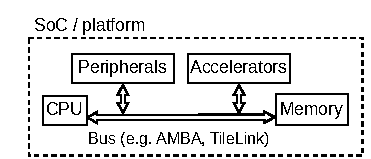
\includegraphics[width=0.8\columnwidth]{figures/exampleplatform/exampleplatform.pdf}
    \end{center}
    \vspace*{-1em}
    \caption{\label{fig:exampleplatform}
        Example SoC platform architecture.
    }
    \vspace*{-1em}
\end{figure}

In this paper, we use the words SoC, system and platform interchangeably to refer to the integrated circuit that integrates various components, including CPUs, memory, and peripherals, as illustrated in Fig.~\ref{fig:exampleplatform}.
The communication between these components is typically managed through standardized bus protocols, such as AMBA~\cite{arm_amba} or TileLink~\cite{tilelink_spec}.
The bounds of components are not always clear-cut.
For example, Fig.~\ref{fig:verifscopecache} shows that caches can be considered part of the CPU or of the rest of the platform.
For a hardware component, we refer to its \emph{input signals} as the inbound wires, and its \emph{inputs} as the values carried by those wires, and similarly for outputs.

\subsection{Timing side-channels}

Multiple hardware optimizations, such as caches and branch predictors, learn and exploit patterns in program execution to improve performance.
In particular, the execution time of later instructions may depend on the outcome of earlier instructions.
For example, accessing a cache line might be faster if the line has been brought into the cache recently by a prior memory access to a nearby location.
% Timing side channels can result from such optimizations when the timing of a program's execution depends on secret data.
Constant-time programming techniques, such as not using secret data as array indices or loop conditions, aim to ensure that secrets do not influence the execution time of a program through such channels~\cite{OsvikShamirTromer2006CacheAES,AlmeidaEtAl2016CTVerif}.

\subsection{Information Flow Tracking}
\label{subsec:ift}

\begin{figure}[t]
    \begin{center}
    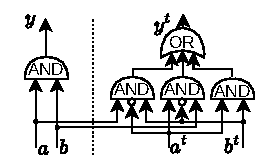
\includegraphics[width=0.5\columnwidth]{figures/glift/glift.pdf}
    \end{center}
    \vspace*{-1em}
    \caption{\label{fig:glift} Taint tracking at gate level~\cite{tiwari2009complete}. Left: original circuit. Right: Added instrumentation for taint tracking. The original input signals are $a$ and $b$. The taint bits corresponding to $a$ and $b$ are respectively $a^t$ and $b^t$. The output taint bit $y^t$ indicates whether the output is tainted, i.e., influenced by the tainted inputs.}
    \vspace*{-1em}
\end{figure}

\begin{figure}[t]
    \begin{center}
    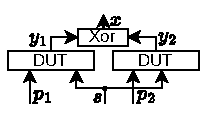
\includegraphics[width=0.5\columnwidth]{figures/miter/miter.pdf}
    \end{center}
    \vspace*{-2em}
    \caption{\label{fig:miter} Miter circuit. The two instances of the same DUT are supplied with the same public data $p$ and unconstrained $s_1$ and $s_2$ secret data. The output bit $y$ (i.e., instantiated for the instances in the miter as $y_1$ and $y_2$) reveals secret data if $x=1$ is satisfiable.}
    % \vspace*{-1em}
\end{figure}

Hardware information flows capture properties such as confidentiality and integrity~\cite{hu2021hardware}.
They are typically tracked using one of two techniques.
The first technique is called dynamic information flow tracking (DIFT).
It captures information flows by augmenting the hardware design under test (DUT) with a synthesizable instrumentation that computes the propagation of taint bits~\cite{tiwari2009complete,ardeshiricham2017register,solt2022cellift,solt2024hybridift,ceesay2024mucfi} as shown in Fig.~\ref{fig:glift}.
The second technique is called a miter circuit.
It captures information flows by comparing the outputs of two copies of the DUT, where all inputs except the sources are unconstrained, while all the others are equal as illustrated in Fig.~\ref{fig:miter}.

\subsection{Hardware-software contracts}
\label{subsec:hw-sw-contracts}

\para{Contract definition}
Hardware-software contracts~\cite{guarnieri2021hardware} split confidentiality responsibilities between the CPU and the software that it executes.
For an initial microarchitectural state, a given program $P$, and the contents of memory containing public information $M_p$ and secret information $M_s$, the contract specifies an execution mode and an observation mode.
The \emph{execution mode} determines which instructions are executed (potentially transiently) and generate events.
The \emph{observation mode} determines which of those events are exposed to an observer (possibly transiently), such as the addresses or values involved in memory accesses.
Under such a contract, the CPU's behavior is summarized as a sequence of observable events known as a hardware trace~\cite{guarnieri2021hardware,oleksenko2022revizor}.

\para{Contract verification}
Multiple independent verification efforts have been conducted to ensure that hardware-software contracts are upheld during program execution, in particular regarding constant-time behavior~\cite{dinesh2024conjunct,ceesay2024mucfi,guarnieri2021hardware,tan2025contractshadowlogic,dinesh2025h,hsiao2024rtl2mmupath,wang2023specification}.
Most techniques consider a fixed contract~\cite{dinesh2024conjunct,ceesay2024mucfi,tan2025contractshadowlogic,dinesh2025h}, while some others leverage custom, non-trivial technique-specific insights to verify a wider variety of contracts~\cite{hsiao2024rtl2mmupath,wang2023specification} using the same technique.

\para{Discussion}
These techniques make assumptions about the platform in which the CPU is integrated, yet there exists no language for formally expressing and verifying them.


%-------------------------------------------------------------------------------
\section{Platform Timing Contracts} \label{sec:reentrant}
%-------------------------------------------------------------------------------
\subsection{Motivational example}

In this section, we first provide a motivational example showing that the integration of a CPU into a platform can introduce new timing channels that were not present in isolation.
We then discuss and formalize reentrant information flows.
Finally, we introduce platform integration contracts to capture these reentrant flows.

\begin{figure}[t]
    \begin{center}
    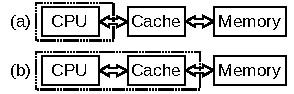
\includegraphics[width=0.6\columnwidth]{figures/verifscopecache/verifscopecache.pdf}
    \end{center}
    \vspace*{-1em}
    \caption{\label{fig:verifscopecache}
        Example verification scopes, represented as dotted boxes. (a: cache excluded) the cache is considered part of the platform. (b: cache included) the cache is considered part of the CPU.
    }
    \vspace*{-1em}
\end{figure}


\para{Methodology (cache excluded)}
Figure~\ref{fig:verifscopecache} (a) illustrates a small system in which a CPU is integrated in a platform that includes a cache and memory.
We instantiate this system, using the Kronos CPU as a case study, and a direct-mapped cache.
We use the state-of-the-art VeloCT~\cite{dinesh2025h} tool to perform constant-time verification of the CPU, which is delimited by the dotted box.
This tool verifies if only instructions of a given "safe instruction set" are executed, then the CPU runtime is independent of their operands.
We consider memory instructions as part of the safe instruction set that should execute in constant-time, in addition to arithmetic RISC-V instructions such as \texttt{add}, \texttt{sub}, \texttt{xor}, etc.

\para{Results (cache excluded)}
The Kronos verification with VeloCT, which indicates that in isolation, the CPU is constant-time secure.
In particular, this result suggests that the timing of any program made of arithmetic and memory instructions does not depend on the data that is processed, even if this data is used as memory addresses.

\para{Methodology (cache included)}
Figure~\ref{fig:verifscopecache} (b) illustrates a scenario similar to Figure~\ref{fig:verifscopecache} (a), but with the cache included in the verification scope, i.e., considered part of the CPU under verification.
Except for this point, we use the same methodology as in the previous cache excluded case.

\para{Results (cache included)}
The Kronos verification with VeloCT, which indicates that this time, the CPU is not constant-time secure.
In particular, this result implies that the program execution timing can depend on secret information used as addresses of memory instructions.

\para{Take-aways}
These results underline that while constant-time verification techniques typically operate at the level of a CPU in isolation (the platform's RTL might not yet be finalized at the CPU verification time), they may not account for all the potential interactions with other components in the system, such as caches or memory.
Therefore, the integration of the CPU into a larger system can introduce new timing channels that were not present in isolation and that are not discovered by existing constant-time verification techniques.

\subsection{Reentrant flows}

We now describe and formalize reentrant information flows, which are at the core of the timing channels that can be introduced by platform integration.

\para{Netlist graphs}
We describe a digital hardware system (e.g., the one illustrated in Figure~\ref{fig:verifscopecache}), as a netlist $G = (V, E)$, where $V$ is the set of vertices representing logic gates such as AND, OR, NOT, flip-flops, adders, and $E$ is the set of directed wires between these vertices.
We denote the subgraph of $G$ that corresponds to the CPU that is integrated in this system as $G_C = (V_C, E_C)$, where $V_C \subseteq V$ and $E_C \subseteq E$.
In particular, for all edges $(u, v) \in E_C$, both $u$ and $v$ are vertices in $V_C$.
We denote the complementary subgraph as $G_{P} = (V_{P}, E_{P})$, where $V_{P} = V \setminus V_C$ and $E_{P} = E \setminus E_C$, corresponding to the platform except the CPU that it integrates.

\para{Constant-time programs \& secret data}
For a given constant-time verification technique, let us denote by $\mathcal{P}$ the set of constant-time programs that are considered for verification.
The elements of the set $\mathcal{P}$ are triples $\tau = (P, M_p, M_s)$, where $P$ is a constant-time program, $M_p$ is the set of public memory valuations, and $M_s$ is the set of secret values that the program may depend on.
Specifically, this set $\mathcal{P}$ depends on the specific constant-time verification technique being used.
For example, for ConjunCT~\cite{dinesh2024conjunct} and VeloCT~\cite{dinesh2025h}, a triple ($P$, $M_p$, $M_s$) is considered constant-time (i.e., part of $\mathcal{P}$) if it contains no so-called "unsafe" instructions, i.e., instructions that can create an operand-dependent timing channel.
For Tan et al.~\cite{tan2025contractshadowlogic}, a triple ($P$, $M_p$, $M_s$) is considered constant-time (i.e., part of $\mathcal{P}$) if it ensures that the program's control flow and all memory accesses are independent of secret data.
The conditions for a program to be constant-time with respect to ConjunCT's and VeloCT's definition are stricter than those of Tan et al.~\cite{tan2025contractshadowlogic}, as the latter generally forbid branches, for instance.
Inclusively more restrictive constraints imply an inclusively smaller set $\mathcal{P}$ of constant-time programs.

\para{Secret propagation}
Constant-time verification techniques generally proceed by analyzing whether the valuation of a state element that captures timing differences can be influenced by secret information.
For example, Tan et al.~\cite{tan2025contractshadowlogic}, LeaVe~\cite{wang2023specification}, ConjunCT~\cite{dinesh2024conjunct} and VeloCT~\cite{dinesh2025h} monitor whether secret information can influence the commit signal, while \ucfi~\cite{ceesay2024mucfi} monitors whether secret information can influence a microarchitectural program counter structure.

We define the \emph{valuation sequence} $\nu$ of a vertex.
For a vertex $v \in V$ and a triple $\tau = (P, M_p, M_s)$, the valuation sequence $\nu_\tau(v)$ is the clock-accurate infinite sequence of valuations that the vertex takes during the execution of a program $P$ with respect to the memory valuations $M_p$ and $M_s$, starting from the CPU's and platform's reset state, assumed deterministic.
Note that we assume determinism for simplicity without loss of generality; to account for non-determinism, we could consider a set $\nu_\tau^{\text{non-det}}(v)$ of all possible valuation sequences instead of a single sequence $\nu_\tau(v)$, without change in the following reasoning.

We denote by $V^s$ the set of vertices in $V$ whose valuation sequence can be influenced by secret information when the system executes a program written in constant-time with respect to the secret data.
An element $v \in V$ belongs to $V^s$ if and only if there exist two triples $\tau = (P, M_p, M_s)$ and $\tau' = (P, M_p, M_s')$ that only differ in $M_s'$, and such that $\tau \in \mathcal{P}$ and $\tau' \in \mathcal{P}$ but $\nu_\tau(v) \neq \nu_{\tau'}(v)$.
We say that a vertex $v \in V$ is \emph{secret-dependent} if it belongs to $V^s$.

For a secret-dependent vertex $v \in V^s$, we define the set $P^s_v$ of \emph{secret propagation paths} to be the paths in the graph $G$ that connect the source of secrets (that can take the value $M_s$ or $M_s'$) to $v$, where all the vertices in the path are secret-dependent.
In particular, $P^s_v$ is non-empty.
Indeed, if $v \in V^s$, then at least one predecessor $u \in V$ of $v$ must also be secret-dependent, which recursively constructs a path in $P^s_u$.

Let us consider a strict subgraph $G' = (V', E') \subsetneq G$ and a vertex $v \in V'^s$.
A path $p$ in $P^s_v$ is said to be \emph{reentrant} in $G'$ if it contains at least one vertex $u \in V \setminus V'$, i.e., a vertex that is outside of $G'$.
Note that this $u$ also belongs to $V^s\setminus V'$ because all nodes in $p$ are secret-dependent by definition of $P^s_v$.
If all paths in $P^s_v$ are reentrant in $G'$, then we say that the vertex $v$ is \emph{fully reentrant} in $G'$.

\para{Example}
Let us consider again the system Figure~\ref{fig:verifscopecache} (a) where $\mathcal{P}$ describes programs where secret data, which is for example initially stored in a well-specified general-purpose register, can be used as the address of a memory instruction.
Because the CPU itself does not contain caches or other components whose timing depends on memory addresses, for $v$ designating the commit signal (for LeaVe~\cite{wang2023specification}, Tan et al.~\cite{tan2025contractshadowlogic}, ConjunCT~\cite{dinesh2024conjunct} or VeloCT~\cite{dinesh2025h}), or a microarchitectural PC signal (\ucfi~\cite{ceesay2024mucfi}), $v$ is fully-reentrant in the CPU, if we consider $G$ being the whole platform, and $G'$ being the CPU.

\subsection{Contracts}

The key idea of our work is to define \emph{platform timing contracts} that capture the possible reentrant information flows in the CPU that are allowed by a given platform.
Since the interface between the output signals of a CPU and the rest of a SoC is usually much simpler than the hardware-software interface, these contracts are expected to be simpler than existing hardware-software contracts.

\para{Interface}
We base our analysis on the widely-studied RISC-V ISA.
The output signals of a RISC-V CPU are all through memory interfaces, which are made of data and control signals.
% \fls{TODO Maybe change all "CPU"'s with "CPU core"}
Data signals transport the data to be read or written to or from the memory.
Control signals transport the information about the memory transaction, such as the memory address, handshake signals, and depending on the memory bus protocol (e.g., AMBA AXI~\cite{arm_amba} or TileLink~\cite{tilelink_spec}), further control signals such as the type of transaction and the size of the data to be read or written.
Input signals of a RISC-V CPU can be more diverse, including memory input data and control signals, interrupt lines, and various other control signals such as clock gating signals.

\para{Platform timing contracts}
Platform timing contracts aim to ensure that state elements that capture timing differences (e.g., a commit signal or a microarchitectural program counter) \emph{are not fully reentrant} in the CPU.
To ensure this, a platform timing contract specifies an upper bound of the information flows between the output signals of the CPU and its input signals.
We express a platform timing contract as a list of rules, listed per CPU output signal.
% In Section~\ref{sec:instrumentation}, we introduce synthesizable constructs that create paths between secret sources and sinks, to ensure that the sets $P^s_v$ are not empty for these sinks, preventing these sinks from being fully-reentrant.
% \textcolor{red}{TODO Continuer ici.}


\para{Example contracts}
Fig.~\ref{fig:contract_equations} provides four example contracts for a RISC-V CPU with a Von Neumann architecture.
We model the memory interface as an outbound address bus (\texttt{addr}), an inbound and an outbound memory data port (respectively \texttt{rdata} and \texttt{wdata}), and a simple valid-ready handshake protocol (inbound \texttt{resp} and outbound \texttt{req}), similar to the \texttt{req} and \texttt{gnt} handshake signals in the Hardware Processing Engines (HWPE) 2.0 interface protocol~\cite{pulpHWPEMem}.
Fig.~\ref{fig:contract_equations}'s contract C1 defines a simple integration contract for a platform with ideal memory that responds with a constant timing (i.e., that is address-independent).
A change in the memory transaction control signals from the CPU can only change the returned value.
Only the request signal (\texttt{req}) can affect the existence, and hence the timing, of a memory response.
% Indeed, a change in the address of a read, for example, might read from a memory cell that contains a different value, and a change, for example in the timing of some request signal will affect the timing of the memory response, and hence the memory read data at some point in time.
The diamond $\lozenge$ underlines that the right-hand side of the implication can happen at any time and for any number of times after the left-hand side.
% \fls{Maybe I should explain more intuitions like why req and addr actually have exactly the same effect.}
Equation~\ref{dict:contract_cache_nointerrupt} adds timing dependence on the memory address, which is typical of structures like caches.
In this contract, \texttt{req} and \texttt{addr} have an identical clause. Indeed, a change in the address of a read, for example, can change a cache miss into a cache hit, changing the timing, and hence the value at some point in time, of the response, including the \texttt{gmt} control signal and the \texttt{rdata} data signals.
Equation~\ref{dict:contract_cache_interrupt} models data-dependent interrupts and timing, which might occur, for example, if some peripheral can be controlled through memory-mapped registers such as an interrupt controller~\cite{riscv_plic_spec_1_0_0}.

\para{Conditional refinements}
\fls{TODO ensure to reference section III.B.}
Equation~\ref{dict:contract_cache_interrupt} implies that writing tainted, i.e., secret, data to memory with a specific address that is not tainted might always trigger an interrupt or affect the timing of the memory response. In some settings, this might be true only for specific address ranges where peripherals are mapped, but parts of the memory address range can typically be used in a data-independent timing.
\fls{Be more concrete here.}
To refine this contract, we introduce address-dependent contracts as in Equation~\ref{dict:contract_cache_interrupt_addressdependent}, where the right-hand side of the implication depends on the memory address set \texttt{periph\_range}, which is a fixed set of addresses.
% Note that the contract could also be refined by making the interrupts dependent on the written data.
% For example, an interrupt might never be triggered, whatever the address, if the written data is zero, for the class of platforms of interest for the CPU integrator.
% In verification, such constraints can be expressed as data-independent timing assuming that the CPU does not write to memory addresses in \texttt{periph\_range} with tainted data.
For example, this can be achieved with RISC-V Physical Memory Protection (PMP) in a setting where the most privileged execution mode does not access secret data and protects the \texttt{periph\_range} address range from being accessed from lower privileges, in the philosophy of trusted execution environments~\cite{lee2019keystone,costan2016sanctum,arm2009trustzone,mcgillion2015opentee,schneider2022sok,bourgeat2018mi6,brasser2022tcx}.

% \fls{TODO Say that we will have a reference contract later for the end-to-end attack.}
% \fls{TODO Say the right-hand side can be anytime after, and for any number of time. Maybe write this as an LTL formula.}


\begin{figure}
    \begin{center}
    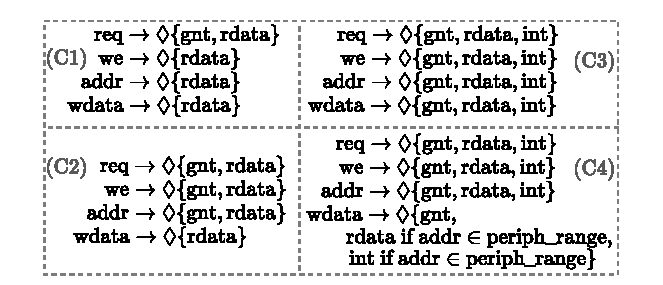
\includegraphics[width=\columnwidth]{figures/contract_equations/contract_equations.pdf}
    \end{center}
    \vspace{-1.8em}
    \caption{Example platform contracts.}
    \label{fig:contract_equations}
    \vspace*{-1.5em} 
\end{figure}

% \begin{equation}
% \label{dict:contract_nocache}
% \begin{array}{rcl}
% \text{req} & \rightarrow & \lozenge \{ \text{gnt}, \text{rdata}\} \\
% \text{we} & \rightarrow & \lozenge \{\text{rdata}\} \\
% \text{addr} & \rightarrow & \lozenge \{ \text{rdata}\} \\
% \text{wdata} & \rightarrow & \lozenge \{ \text{rdata} \} \\
% \end{array}
% \end{equation}

% \begin{equation}
% \label{dict:contract_cache_nointerrupt}
% \begin{array}{rcl}
% \text{req} & \rightarrow & \lozenge \{ \text{gnt}, \text{rdata}\} \\
% \text{we} & \rightarrow & \lozenge \{ \text{gnt}, \text{rdata}\} \\
% \text{addr} & \rightarrow & \lozenge \{ \text{gnt}, \text{rdata}\} \\
% \text{wdata} & \rightarrow & \lozenge \{ \text{rdata} \} \\
% \end{array}
% \end{equation}

% \begin{equation}
% \label{dict:contract_cache_interrupt}
% \begin{array}{rcl}
% \text{req} & \rightarrow & \lozenge \{ \text{gnt}, \text{rdata}, \text{interrupt}\} \\
% \text{we} & \rightarrow & \lozenge \{ \text{gnt}, \text{rdata}, \text{interrupt}\} \\
% \text{addr} & \rightarrow & \lozenge \{ \text{gnt}, \text{rdata}, \text{interrupt}\} \\
% \text{wdata} & \rightarrow & \lozenge \{ \text{gnt}, \text{rdata}, \text{interrupt} \} \\
% \end{array}
% \end{equation}

% \begin{equation}
% \label{dict:contract_cache_interrupt_addressdependent}
% \begin{array}{rcl}
% \text{req}  & \rightarrow & \lozenge \{ \text{gnt}, \text{rdata}, \text{interrupt}\} \\
% \text{we}  & \rightarrow & \lozenge \{ \text{gnt}, \text{rdata}, \text{interrupt}\} \\
% \text{addr} & \rightarrow & \lozenge \{ \text{gnt}, \text{rdata}, \text{interrupt}\} \\
% % \text{wdata} & \rightarrow & \lozenge \{ \text{rdata}, \text{interrupt} \} \\
% \text{wdata} & \rightarrow & \lozenge \{ \text{rdata}, \\
% & & \text{gnt if addr in periph\_range} \\
% & & \text{interrupt if addr in periph\_range} \} \\

% \end{array}
% \end{equation}

\para{Ordering of \pics}
Like for sinks, we can define a partial ordering of \pics.
We say that a contract A is (inclusively) stronger than a contract B if for every output of the CPU (i.e., the left-hand side of the arrow in the contract), the set of possible CPU inputs tainted by this output in contract A is a subset of the set of possible CPU inputs tainted by this output in contract B.
Said otherwise, contract A is stronger than contract B if it allows for fewer possible information flows.
For example, Equation~\ref{dict:contract_cache_interrupt_addressdependent} is stronger than Equation~\ref{dict:contract_cache_interrupt}, and Equation~\ref{dict:contract_cache_nointerrupt} is stronger than Equation~\ref{dict:contract_cache_interrupt}.
A CPU that is verified to have a constant-time behavior with respect to a stronger \pic is also verified with respect to a weaker \pic.

\begin{figure}
    \begin{center}
    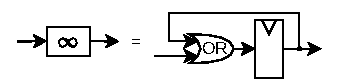
\includegraphics[width=.7\columnwidth]{figures/stickyone/stickyone.pdf}
    \end{center}
    \vspace*{-1em}
    \caption{Sticky-one operator. The sticky-one is reset to zero (not illustrated in the figure) and sticks to 1 once it is set.}
    \label{fig:stickyone}
    \vspace*{-.4em}
\end{figure}


\begin{figure}[t]
    \begin{center}
    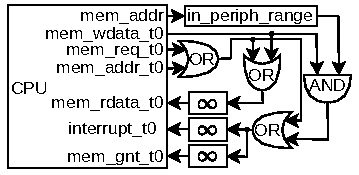
\includegraphics[width=.7\columnwidth]{figures/picinstrum_taints/picinstrum_taints.pdf}
    \end{center}
    \vspace*{-1em}
    \caption{\Pici for a design whose information flows are tracked with dynamic information flow tracking instrumentation. Signals that end with \texttt{t0} represent the taint signals~\cite{tiwari2009complete,solt2022cellift}.
    }
    \label{fig:pic_instrum_taints}
    \vspace*{-.4em}
\end{figure}

\begin{figure}[t]
    \begin{center}
    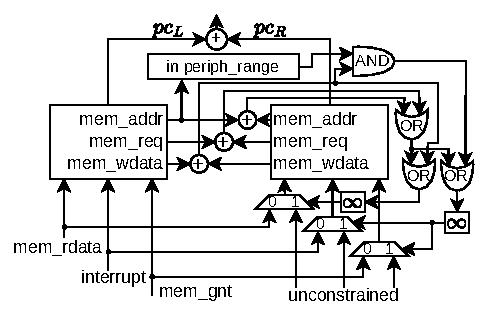
\includegraphics[width=0.9\columnwidth]{figures/picinstrum_miter/picinstrum_miter.pdf}
    \end{center}
    \vspace*{-1em}
    \caption{\Pici for a design whose information flows are tracked with a miter. }
    \label{fig:pic_instrum_miter}
    \vspace*{-.4em}
\end{figure}


%-------------------------------------------------------------------------------
\section{Instrumentation} \label{sec:instrumentation}
%-------------------------------------------------------------------------------

% \fls{TODO Continue here}
In this section, we express these contracts as a synthesizable \pici (\PICI).
Because it is an information flow property, the \PICI cannot be directly applied to the CPU under verification.
Indeed, in the original CPU before IFT instrumentation or miter construct, the notion of taint~\cite{solt2022cellift,ceesay2024mucfi} or two-trace property~\cite{wang2023specification,dinesh2024conjunct,dinesh2025h,tan2025contractshadowlogic} does not yet exist.
Instead, the \PICI is applied to the construct that supports information flows, which is either a circuit with DIFT instrumentation, or a miter (see Section~\ref{subsec:ift}).

\para{Sticky-one operator}
Fig.~\ref{fig:stickyone} introduces the sticky-one operator, which is a building block of the \PICI.
It models the diamond $\lozenge$ operator in the instrumentations by making its output stick to 1 as soon as its input is 1.
Its output returns to zero only when the system is reset.

\para{\PICI for DIFT}
We first construct the \PICI for CPUs instrumented for DIFT~\cite{tiwari2009complete,solt2022cellift}.
We materialize contract information flows (i.e., arrows ``$\rightarrow$'' in a given contract) from a CPU output signal to a CPU input signal as a wire between the two corresponding taint signals, where a sticky-one operator accommodates for information flows that might return later (i.e., the $\lozenge$ operator).
When multiple CPU outputs have a contract information flow to a single CPU input signal (i.e., there are several arrows ``$\rightarrow$'' in the contract whose right-hand set contains the same input signal), the corresponding taint signals are \texttt{OR}'ed together, meaning that the input signal can be influenced by any of these output signals.
The \PICI for Contract C4 is shown in Fig.~\ref{fig:pic_instrum_taints} when relying on DIFT instrumentation.

\para{\PICI for miter constructs}
\fls{TODO Continue here.}
We first construct the \PICI for a CPU that relies on a miter construct, the \PICI must ensure that the CPU input signals that are influenced by the CPU output signals are distinct between the two copies of the CPU.
This is achieved using \texttt{XOR} operations between the CPU outputs of the two copies.
Ultimately, another \texttt{XOR} operation with the result of this difference is performed with the input signal, deciding whether for a given input signal, the two copies of the CPU will receive the same input, or one copy will receive a flipped input.
Note that there is no conceptual difference between the \PICI for a DIFT instrumentation and the \PICI for a miter construct, yet the former benefits from the abstraction built into the DIFT instrumentation, which allows for a more compact and arguably more intuitive \PICI.
\fls{TODO Reference figure 8.}

% \para{Take-away}
% In Section~\ref{sec:eval}, we will show that when instrumented with the \PICI, the techniques that were originally unable to detect basic timing side-channels due to the verification scope not including caches are now able to detect them.
% Importantly, this requires no change to the verification technique implementation at all, as the \PICI becomes part of the design under verification's taint tracking logic or miter construct from the verification tool's perspective.
% In terms of performance, we will also show that adding the \PICI incurs a negligible overhead.
% However, while the \PICI addresses a necessary condition for maintaining soundness when the CPU under verification is integrated in a system, existing automated constant-time verification tools have other critical shortcomings that affect unsoundness besides platform integration, as we show next in Section~\ref{sec:techniques}.

%-------------------------------------------------------------------------------
\section{Evaluation} \label{sec:evaluation}
%-------------------------------------------------------------------------------
In this section, we first present the \PICI implementation (Section~\ref{subsec:pici_impl}), evaluate its performance and the resulting soundness improvement (Section~\ref{subsec:pici_platform_eval}), and finally verify the compliance of several platforms to the \pics discussed in this paper (Section~\ref{subsec:pici_platform_verif}).
% For comprehensiveness, we then also  verify that not only the CPU, but also the rest of the platform complies with its own contract terms, i.e., that a platform will not propagate more taint than what the contract stipulates~(Section~\ref{subsec:pici_platform}).

\para{Evaluation setup}
We execute the performance evaluations on a server equipped with an Intel Xeon E5-2667 CPU with 256\,GB RAM.
We use the 2-stage Sodor CPU~\cite{sodor} (commit \texttt{32d49f9}) and the 3-stage Kronos CPU~\cite{kronos} (commit \texttt{13678d4}), which are simple RISC-V CPUs already used in previous constant-time verification benchmarks~\cite{wang2023specification,tan2025contractshadowlogic,ceesay2024mucfi}.

% \para{The problem with a CPU in isolation}
% We now show that techniques can be unsound because the SoC integration is not considered.
% In particular, we show that \ucfi~\cite{ceesay2024mucfi} and VeloCT~\cite{dinesh2025h} call instructions safe, but these instructions are not safe when the CPU is integrated into a platform that contains a cache.
% We execute \ucfi and VeloCT on the 2-stage Sodor RISC-V CPU~\cite{sodor} (commit \texttt{32d49f9}) and ask whether loads and stores are safe instructions, which the two techniques answer positively because they do not consider reentrant information flows.

% We introduce a simple SoC architecture composed of a Sodor CPU, a set-associative cache and memory as depicted in Fig.~\ref{fig:simple_soc}.
% We mount a cache attack on the SoC, where we measure the timing differences in cache access patterns when secret data is used as an address, and we obtain different timing results depending on whether the secret data causes a hit or a miss in the cache.
% As a result of this experiment, we indeed observe differences in the timing of the memory accesses between a hit and a miss using exclusively instructions that \ucfi and VeloCT considers safe.
% This demonstrates that instructions that were considered safe by some techniques are not necessarily safe when the CPU is integrated into a platform that contains a cache.
% This justifies the need for \pics, which model an upper bound for reentrant information flows through the platform.

\subsection{\PICI implementation}
\label{subsec:pici_impl}

The limited interface between the CPU and the platform makes the \PICIs simple, as earlier illustrated in Fig.~\ref{fig:pic_instrum_taints} and Fig.~\ref{fig:pic_instrum_miter}.
We implement a Yosys synthesizer pass~\cite{wolf2013yosys} that instruments a CPU that is either instrumented with taint tracking logic such as GLIFT~\cite{tiwari2009complete} or CellIFT~\cite{solt2022cellift}, or part of a miter construct.
The synthesizer pass takes as input a Verilog description of the CPU under test in one of these two configurations (instrumented for taint tracking or in a miter) and outputs a Verilog design instrumented with the \PICI.
In addition to the CPU's Verilog description, the synthesizer pass takes a conditional contract as input, with a syntax similar to the one used in Fig.~\ref{fig:contract_equations}, and takes a machine-readable description of the CPU's interface ports.
The instrumentation process takes a few seconds, including the boilerplate time taken by Yosys to process the designs.
% The \PICI synthesizer pass is made of around 500 lines of C++ code.
% \fls{TODO: Give an example contract in appendix and of the CPU interface ports file.}

\begin{figure}[t]
    \begin{center}
    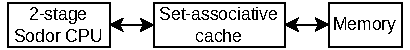
\includegraphics[width=0.80\columnwidth]{figures/simple_soc/simple_soc.pdf}
    \end{center}
    \vspace*{-1.2em}
    \caption{\label{fig:simple_soc} Simple SoC architecture with a CPU, a cache, and memory.}
    \vspace*{-1.4em}
\end{figure}

\begin{table}[t]
    \vspace*{1.2em}
    \centering
    \caption{Verification results for the original (O) Sodor and Kronos, and for \PICI-instrumented (P) Sodor and Kronos for Contract C3. Results are ``pass'' if all memory instructions are considered safe with regard to all their operands (in particular with regard to the address).
    Time indicates the time to obtain a proof for a subset of instructions that excludes memory instructions if they are shown to be non-constant-time.
    The time shown for \ucfi is the mean across instructions.}
    \vspace*{-.4em}
    \small
    \begin{tabular}{|c|c|c|c|c|}
        \hline
        \rowcolor{gray!20}
        & \multicolumn{2}{c|}{\textbf{\ucfi}} & \multicolumn{2}{c|}{\textbf{VeloCT}} \\
        \hline
        \rowcolor{gray!10}
        & \textbf{Sodor} & \textbf{Kronos} & \textbf{Sodor} & \textbf{Kronos} \\
        \hline
        Time (O) & 8\,min & 31\,min & 1\,min & 1\,min \\
        \hline
        Result (O) & Pass \textcolor{green}{\gcheck} & Pass \textcolor{green}{\gcheck} & Pass \textcolor{green}{\gcheck} & Pass \textcolor{green}{\gcheck} \\
        \hline
        Time (P) & 8\,min & 31\,min & 1\,min & 1\,min \\
        \hline
        Result (P) & Fail \textcolor{red}{\rcross} & Fail \textcolor{red}{\rcross} & Fail \textcolor{red}{\rcross} & Fail \textcolor{red}{\rcross} \\
        \hline
    \end{tabular}
    \vspace*{-.4em}
    \label{tab:verif_results_simple_soc}
\end{table}



\subsection{Soundness improvement with \PICI}
\label{subsec:pici_platform_eval}

We have shown in Section~\ref{sec:reentrant:motivational} that the security guarantees provided by VeloCT, and similarly with \ucfi, may not hold when the CPU is integrated into a platform that contains elements with address-dependent timing such as caches.
% Sodor is a simple CPU core that belongs to LeaVe's and CSL's constant-time verification testbench.
% \fls{Abrupt introduction of Sodor.}
We first verify Sodor and Kronos with \ucfi and VeloCT (ConjunCT is not open-source but its authors affirmed that it is superseded by VeloCT).
We then instrument Sodor and Kronos with the \PICI and verify them again.
We report the verification results, as well as the time taken by each tool to formulate a proof in Table~\ref{tab:verif_results_simple_soc}.
The difference in verification time with and without the \PICI is not significant.
We observe that the \PICI indeed can correct the unsoundness of \ucfi and VeloCT with regard to the platform integration such as cache side channels.

% \begin{table}[t]
%     \centering
%     \caption{Verification of the compliance of platforms to \PICI. SimpleSoC is depicted in Fig.~\ref{fig:simple_soc}, exempt of Sodor.}
%     \small
%     \begin{tabular}{|l|c|c|}
%         \hline
%         \rowcolor{gray!20} % Color for the table header
%         & \textbf{SimpleSoC} & \textbf{Caliptra} \\
%         \hline
%         Time  (Contract A) & \textcolor{red}{TODO Measure} & \textcolor{red}{TODO Measure} \\
%         \hline
%         Result (Contract A) & Pass & Fail \\
%         \hline
%         Time  (Contract B) & \textcolor{red}{TODO Measure} & \textcolor{red}{TODO Measure} \\
%         \hline
%         Result (Contract B) & Pass & Pass \\
%         \hline
%         Time  (Contract C) & \textcolor{red}{TODO Measure} & \textcolor{red}{TODO Measure} \\
%         \hline
%         Result (Contract C) & Fail & Pass \\
%         \hline
%     \end{tabular}
%     \label{tab:verif_platform_compliance_results}
% \end{table}

\begin{table}[t]
    \centering
    \caption{Verification of the compliance of platforms to \PICI.}
    \vspace*{-.4em}
    \small
    \begin{tabular}{|c|c|c|c|}
        \hline
        \rowcolor{gray!20} % Color for the table header
        \textbf{Contract} & \texttt{nocache} & \texttt{cache} & \texttt{interrupt} \\
        \hline
        C1 & Pass \textcolor{green}{\gcheck} & Fail \textcolor{red}{\rcross} & Fail \textcolor{red}{\rcross} \\
        \hline
        C2 & Pass \textcolor{green}{\gcheck} & Pass \textcolor{green}{\gcheck} & Fail \textcolor{red}{\rcross} \\
        \hline
        C3 & Pass \textcolor{green}{\gcheck} & Pass \textcolor{green}{\gcheck} & Pass \textcolor{green}{\gcheck} \\
        \hline
        C4 & Pass \textcolor{green}{\gcheck} & Pass \textcolor{green}{\gcheck} & Fail \textcolor{red}{\rcross} \\       \hline
    \end{tabular}
    \label{tab:verif_platform_compliance_results}
    \vspace*{-.4em}
\end{table}


\subsection{Platform verification}
\label{subsec:pici_platform_verif}

Finally, we verify the compliance of the platform with the \pic.
Because these contracts specify a form of non-interference, they can be verified conveniently with miter constructs, similar to how most techniques verify constant-time properties for CPUs~\cite{dinesh2024conjunct,dinesh2025h,wang2023specification,tan2025contractshadowlogic}.
We verify three platforms.
The \texttt{cache} platform is a simple SoC architecture composed of a CPU, a set-associative cache and memory, as depicted in Fig.~\ref{fig:simple_soc}.
The \texttt{nocache} platform is like the \texttt{cache} platform, but the cache is removed, connecting the CPU directly to the memory, which is modeled as having no address-dependent latency.
The \texttt{interrupt} platform is like the \texttt{cache} platform, but also adds an uncached interrupt controller at the address \texttt{0x1000}, which generates an interrupt signal when a non-zero value is written to this address.
For each of these platforms, we verify Contracts C1-C4 where we constrain \texttt{periph\_range} to be \texttt{0x1000} to \texttt{0x1000}, and Contract D that is like Contract C but with a \texttt{periph\_range} of \texttt{0x2000} to \texttt{0x2FFF}.
% \fls{TODO Check the mem range for Caliptra.}
% \fls{TODO Say that the caliptra contract proves that the ICCM and DCCM indeed do not have timing side channels, as expected}
We construct miters whose designs under test is the platform seen from the CPU's perspective, i.e., whose inputs are the outputs of the CPU, and whose outputs are the inputs of the CPU.
Note that the CPU itself is not part of this miter.
To verify, for example, the last arrow of Contract C4, we enforce all inputs of the miter to be identical between the two sides of the miter except for the \texttt{mem\_wdata} input, and we additionally constrain the \texttt{mem\_addr} input, identical between the two sides of the miter, not to be in the \texttt{periph\_range} range.
We then verify that only \texttt{mem\_rdata} can be affected by changes to \texttt{mem\_wdata} by \texttt{xor}'ing the outputs of \texttt{mem\_gnt} for the two copies of the platform in the miter together and expressing a SAT formula on this signal, which should never be set.
Table~\ref{tab:verif_platform_compliance_results} summarizes the verification results obtained with Cadence Jaspergold for the different platforms.
The total duration of the experiment does not exceed one minute.


%-------------------------------------------------------------------------------
\section{Discussion} \label{sec:discussion}
%-------------------------------------------------------------------------------
ISAs like RISC-V~\cite{riscv_privileged} communicate with the rest of the system through memory interfaces.
Some other ISAs like x86~\cite{intel_x86_manual} have special I/O instructions that are not memory-mapped.
The reasoning about \pics for these ISAs would need to account for the different ways in which they interact with the system and might incur more clauses in the contracts to account for these two separate channels for communicating with the system.
System-level instructions of ISAs like MIPS~\cite{mips_isa} (e.g., the \texttt{mfc0} instruction) or ARM~\cite{armv8_isa} (e.g., the \texttt{SVC} instruction) also require additional ports to include into contracts to describe how the system might react.


%-------------------------------------------------------------------------------
\section{Related Work} \label{sec:related}
%-------------------------------------------------------------------------------
Previous work has proposed means of mitigating some platform-related side channels such as cache timing attacks~\cite{kar2023mitigating,saileshwar2021mirage,giner2023scatter,werner2019scattercache,qureshi2018ceaser} or network on chip interference~\cite{wassel2013surfnoc,wang2012efficient,schoeberl2012statically,wassel2014networks,psarras2015phasenoc,alonso2019low,sadeghi2019toward,shalaby2021sentry}.
Our work is orthogonal to these works and models a platform that is tolerated to have a specific set of potential side channels.
Hardware-software contracts and some constant-time techniques~\cite{guarnieri2021hardware,wang2023specification,tan2025contractshadowlogic} typically consider the assumption that addresses of memory operations might eventually influence timing.
But not all platforms will have such flows, and some platforms will also create reentrant timing flows from other CPU output signals as discussed in Section~\ref{sec:reentrant}.
The \PICI that we introduce proposes fine-grained platform integration contracts, and makes them synthesizable so that they can directly be used upon techniques that are unaware of reentrant information flows as shown in Section~\ref{subsec:pics_eval}.


%-------------------------------------------------------------------------------
\section{Conclusion} \label{sec:conclusion}
%-------------------------------------------------------------------------------
We introduced platform timing contracts as an extension of hardware-software contracts.
They provide a language for specifying expected timing channels in full-system contexts rather than isolated CPUs.
To make such reasoning compatible with existing CPU timing side-channel verification frameworks, we proposed an instrumentation that accounts for platform-specific timing effects.
Our evaluation shows a negligible verification performance overhead while uncovering timing channels that would otherwise remain invisible in isolation.


\newpage

\bibliographystyle{IEEEtran}
\bibliography{main.bib}

\end{document}
